\documentclass[11pt]{article}

\usepackage[a4paper,margin=29mm]{geometry}
\usepackage[T1]{fontenc}
\usepackage{lmodern}
\usepackage{microtype}
\usepackage{amsmath,amssymb,amsthm,mathtools}
\usepackage{booktabs}
\usepackage{array}
\usepackage{longtable}
\usepackage{float}
\usepackage{enumitem}
\usepackage{tikz}
\usepackage[hidelinks]{hyperref}

\newtheorem{theorem}{Theorem}[section]
\newtheorem{proposition}[theorem]{Proposition}
\newtheorem{corollary}[theorem]{Corollary}
\newtheorem{lemma}[theorem]{Lemma}
\theoremstyle{definition}
\newtheorem{definition}[theorem]{Definition}
\newtheorem{problem}[theorem]{Problem}
\theoremstyle{remark}
\newtheorem{remark}[theorem]{Remark}

\newcommand{\PG}{\mathrm{PG}}
\newcommand{\F}{\mathbb{F}}
\newcommand{\cC}{\mathcal{C}}
\newcommand{\cU}{\mathcal{U}}
\newcommand{\A}{A_5}

\title{A conic deep-hole syndrome locus characterizes the Clebsch code}
\author{Tavis Rudd}
\date{July 2026}

\begin{document}
\maketitle

\begin{abstract}
Let $A$ be a six-arc in $\PG(2,11)$, and let $\cU(A)$ be the projective
points lying on no chord of $A$.  For the associated $[6,3,4]_{11}$ MDS
code, $\cU(A)$ is its projective deep-hole syndrome locus.  We prove that
$\cU(A)$ lies on a conic if and only if $A$ is projectively equivalent to
the Clebsch hexagon; in that case $\cU(A)$ is exactly a nonsingular conic.
Thus this coarse decoding condition characterizes the non-GRS Clebsch code
up to monomial equivalence.  The uncovered conic determines the associated
polarity, and Dye's theorem then identifies the stabilizer as $A_5$;
neither structure is assumed.  An exact census strengthens this result:
the same characterization holds when conic containment is weakened to
containment in the zero set of some nonzero form of degree at most three.

For the Clebsch code, the conic equation tests syndrome distance, and
decoder ambiguity recovers the Brianchon geometry and an invariant
bipartition of the three-coordinate supports.  The conceptual tool is a
universal chord-defect identity.  Together with passant counts, it reduces
the classification of $k$-arcs whose uncovered locus is a nonsingular
conic to exact terminal searches.  For $4\le k\le8$, only a projective
four-frame over $\F_5$ and the Clebsch hexagon over $\F_{11}$ occur.
Equivalently, these give the only projective $[k,k-3,4]_q$ MDS codes in
this range whose projective distance-three syndrome locus is a nonsingular
conic.
\end{abstract}

\noindent\textbf{Keywords.} Clebsch hexagon; MDS code; deep hole; finite
projective plane; arc; conic.

\smallskip
\noindent\textbf{2020 Mathematics Subject Classification.} 51E21, 94B05,
51E22, 05B25.

\section{Introduction}
\label{sec:intro}

The complete nearest-codeword structure of a code can retain geometry that
is absent from its definition.  The example here is a non-GRS
$[6,3,4]_{11}$ MDS code.  Its maximum-distance syndrome directions form a
conic, and that coarse locus already determines the projective code: its six
parity-check columns are projectively equivalent to the Clebsch hexagon,
with the associated polarity and $A_5$ symmetry.  No conic, polarity, group
action, or classical hexagon structure is assumed.  Thus the problem is an
inverse one: when does the projective deep-hole locus determine an MDS code,
and how much of its geometry can nearest-codeword data recover?

Let $C$ be a linear $[n,k,d]_q$ code with covering radius $\rho$ and
full-rank parity-check matrix $H$. For a received word $v$, write
$\sigma(v)=Hv^{\mathsf T}$ and
\[
 w(s)=\min\{\operatorname{wt}(e):He^{\mathsf T}=s\}.
\]
Then $d(v,C)=w(\sigma(v))$, and $v$ is a \emph{deep hole} precisely when
this minimum is $\rho$. The syndrome $s$ specifies one coset of $C$, whose
coset leaders are its weight-$w(s)$ representatives. Because
$w(\lambda s)=w(s)$ for $\lambda\ne0$, maximum-distance syndrome directions
form a projective locus
\[
 \mathcal D_{\mathrm{proj}}(C)=
 \{[s]\in\PG(n-k-1,q):w(s)=\rho\}.
\]
Thus one projective direction represents $q-1$ distinct nonzero syndrome
cosets, while each coset contains $|C|$ received words.

For an MDS code of redundancy $r=n-k$, the parity-check columns form a
projective arc in $\PG(r-1,q)$, and $w(s)$ is the least number of columns
whose span contains $[s]$. Adjoining a new column preserves the MDS property
exactly when its direction avoids every hyperplane spanned by $r-1$ existing
columns. In the redundancy-three plane case used here, this specializes to
weights one, two, or three according as the direction lies on the arc, on a
secant of the arc, or on neither; an extension point is precisely a direction
missed by every secant. We write $\cU(A)$ for this extension locus. If
$\cU(A)\ne\emptyset$, then the associated code has covering radius three
and $\cU(A)=\mathcal D_{\mathrm{proj}}(C)$. This dictionary is classical in
the theory of complete arcs and is developed for MDS codes by Davydov,
Marcugini, and Pambianco~\cite{DMP2021}; their Theorem~6.3 supplies the
leader count used in Section~\ref{sec:code}. See also
Hirschfeld~\cite{Hirschfeld1998} for the plane arc/covering-radius setting.
We call $A$ \emph{conic-filling} when $\cU(A)$ is the full
$\F_q$-rational point set of a nonsingular conic.

\begin{theorem}[Rigidity theorem]
\label{thm:rigidity}
For a six-arc $A\subset\PG(2,11)$, the following are equivalent:
\begin{enumerate}[label=(\roman*),leftmargin=2em]
\item the uncovered locus $\cU(A)$ lies on some conic (possibly
degenerate);
\item $\cU(A)$ is exactly the set of $\F_{11}$-points of a nonsingular
conic;
\item $A$ is $\mathrm{PGL}(3,11)$-equivalent to the Clebsch hexagon.
\end{enumerate}
\end{theorem}

The proof reconstructs the hexagon from conic containment alone.
A line bound, a chord-defect identity, and Dye's Brianchon theorem give the
conceptual implication. Finite enumeration supplies the low-degree
strengthening and quantitative clauses.  The same geometry then gives an
exact distance oracle and all nearest-codeword multiplicities. Its
ambiguity strata reconstruct the Brianchon points, the self-polar triangles,
and the invariant support bipartition.
The Lean development checks the central deductions conditional on two
classical inputs from Dye; the low-degree, gap, and terminal small-arc
claims instead use separately replayable exact enumeration.

The chord-defect identity has a second role independent of the Clebsch
classification.  For a Clebsch hexagon $K$ it gives
$|\cU(K)|=q^2-14q+45$, with off-conic excess $(q-4)(q-11)$ when
$q\equiv3\pmod4$.  For an arbitrary conic-filling $k$-arc, the same moment
calculation forces $q$ odd and
$2k-3\le q<\binom{k}{2}$, together with a sharper quadratic barrier.  We
classify the cases through eight points.

The configuration goes back to Clebsch~\cite[p.~336]{Clebsch1871}. Edge
constructed its finite-plane form and determined its order-$60$ stabilizer
\cite[\S\S29--32]{Edge1956}; Dye proved projective uniqueness and determined
the stabilizer over a general field~\cite[Theorems~1 and 3,
pp.~275--278]{Dye1991}; Storme and Van~Maldeghem identified the corresponding
six-arc in their finite-plane classification~\cite{SVM1995}. Deep holes of
Reed--Solomon codes have both an algorithmic history
\cite{GuruswamiVardy2005,ChengMurray2007} and a geometric classification in
the projective case~\cite{ZWK2020}. Those results concern GRS codes, whose
arcs lie on normal rational curves; the code here is not GRS.

\paragraph{What is new and what is not.} The hexagon, its uniqueness and
stabilizer, and its complete-exterior-set interpretation are classical
\cite{Clebsch1871,Edge1956,Dye1991,BSW1992,SVM1995}. Sadeh classified the
six-arcs of $\PG(2,11)$~\cite{SadehThesis1984}; we claim no priority for
that census or its extension counts. We prove the conic-locus identification
of Proposition~\ref{prop:deep-holes-conic} directly here. The new
contribution is the symmetry-free coding
criterion and its consequences: low-degree rigidity, quantitative gaps,
leader-support bipartition, decoder reconstruction, and the finite-field boundary.

\section{The Clebsch hexagon}
\label{sec:hexagon}

Fix the nonsingular conic
\[
 \cC:\ XZ=Y^2
\]
in $\PG(2,11)$, with its $12$ points identified with $\PG(1,11)=\F_{11}\cup\{\infty\}$
in the usual way. The stabilizer of $\cC$ in $\mathrm{PGL}(3,11)$ is
$\mathrm{PGL}_2(11)$, acting on $\cC$ as it acts on the projective line.

A convenient representative is
\[
 A=\{(1,10,0),\,(1,9,1),\,(1,4,7),\,(1,8,5),\,(0,1,4),\,(1,1,7)\}.
\]
It is a six-arc disjoint from $\cC$; its fifteen joins also avoid $\cC$.
The following invariant construction explains its symmetry.

\begin{definition}[Clebsch hexagon]
\label{def:hexagon}
Let $\A\subset\mathrm{PGL}_2(11)$ be an icosahedral subgroup. The
six Sylow $5$-subgroups of $\A$ each fix two points of $\cC$. The
\emph{Clebsch hexagon} is the set of poles of the six chords joining these
fixed pairs. More generally, following Dye, a Clebsch hexagon over a field
is a six-arc with exactly ten nonvertex triple-chord concurrence points,
called its Brianchon points.
\end{definition}

For a nonsingular conic over an odd field, an \emph{external point} lies on
two tangents and an \emph{internal point} on none; an \emph{exterior}, or
\emph{passant}, line is disjoint from the conic.
Edge's six vertices are external, their fifteen joins are exterior, and
those joins concur three at a time at ten internal Brianchon
points~\cite[\S\S29--32]{Edge1956}. Thus the hexagon is a complete exterior
set in the terminology of Blokhuis, Seress, and Wilbrink
\cite[pp.~143,146]{BSW1992}. Their $q=11$ list also contains a Pasch
configuration, but its four collinear triples prevent it from defining an
MDS code. Thus exteriority alone gives only
$\cC(\F_{11})\subseteq\cU(A)$; the arc hypothesis selects the Clebsch
branch, and Proposition~\ref{prop:deep-holes-conic} proves equality.

The displayed hexagon is the arc $K_2$ of Storme and Van~Maldeghem
\cite[Props.~11--12]{SVM1995} and Dye's synthetic hexagon when $5$ is a
square in the base field~\cite[Theorem~1, pp.~275--276]{Dye1991}. At
characteristic $11$, Dye's Theorems~1--3 give projective uniqueness, the
unique associated polarity, and stabilizer $A_5$; in the displayed
coordinates the associated conic is $\cC$
\cite[pp.~275--278]{Dye1991}. His calculation also shows that the six
vertices lie on no conic in characteristic $11$
\cite[Theorem~2, pp.~277--278; p.~281]{Dye1991}. Storme and Van~Maldeghem
record that the arc is incomplete at $q=11$~\cite[Prop.~13]{SVM1995}, so
the associated redundancy-three code has covering radius three.

\section{A universal chord-defect identity}
\label{sec:chord-defect}

\begin{theorem}[Universal chord defect]
\label{lem:chord-defect}
Let $A$ be a $k$-arc in $\PG(2,q)$ with $k\ge4$. Let $n_i$ count the
off-arc points incident with exactly $i$ chords, put
\[
 r=\lfloor k/2\rfloor,\qquad
 t(A)=\sum_{i=3}^{r}\binom{i-1}{2}n_i,
\]
and write $m=\binom{k}{2}$. Then
\[
\begin{aligned}
 |\cU(A)|&=q^2-(m-1)q+
 \left(m+3\binom{k}{4}-k+1\right)-t(A),\\
 0\le t(A)&\le3\binom{k}{4}\frac{r-2}{r},
 \qquad k\le5\Longrightarrow t(A)=0.
\end{aligned}
\]
\end{theorem}

\begin{proof}
At a point off $A$, concurrent chords have pairwise disjoint endpoint
pairs, so at most $r$ chords occur. Counting chord--point incidences and
pairs of disjoint chords gives
\[
 \sum_i i n_i=m(q-1),\qquad
 \sum_i\binom{i}{2}n_i=3\binom{k}{4}.
\]
Since $\binom{i}{2}=(i-1)+\binom{i-1}{2}$, the number of covered off-arc
points is $m(q-1)-3\binom{k}{4}+t(A)$. Subtraction from the
$q^2+q+1-k$ off-arc points proves the identity. Finally,
\[
 \binom{i-1}{2}\le\frac{r-2}{r}\binom{i}{2}\qquad(3\le i\le r),
\]
and the second moment gives the defect bound.
\end{proof}

\begin{corollary}[Conic-filling window and six-arcs]
\label{cor:conic-filling-window}
If $|\cU(A)|=q+1$, then
\[
 t(A)=q^2-mq+m+3\binom{k}{4}-k,\qquad
 q^2-mq+m-k+\frac{6}{r}\binom{k}{4}\le0,
\]
and $q<m$. Under the same hypothesis $|\cU(A)|=q+1$, if $q$ is even,
then $\cU(A)$ is not an arc. Hence if
$\cU(A)$ is a nonsingular conic, then $q$ is odd and
\[
 2k-3\le q<\binom{k}{2}.
\]
For $k=6$, writing $c(A)=n_3$ gives
\[
 |\cU(A)|=q^2-14q+55-c(A),\qquad
 0\le c(A)\le15,\qquad
 c(A)=(q-6)(q-9)
\]
when $|\cU(A)|=q+1$. For the displayed Clebsch hexagon, Dye's ten
Brianchon points give $c(A)=10$; its fifteen chords have $45$ disjoint
pairs, cover $115$ of the $127$ off-arc points, and leave exactly twelve
uncovered.
\end{corollary}

\begin{proof}
The first formula is Theorem~\ref{lem:chord-defect} rearranged, and its
comparison with the defect bound gives the quadratic inequality. There are
$q^2-k$ covered off-arc points, so $q^2-k\le m(q-1)$; if $q\ge m$, then
$0\le q(q-m)\le k-m<0$, a contradiction.

Suppose $q$ is even and $\cU(A)$ is an arc. Since it has $q+1$ points, it
has a nucleus $N\notin\cU(A)$ through which every line is tangent
\cite[p.~177]{Hirschfeld1998}. Every chord of $A$ is disjoint from
$\cU(A)$, so no chord contains $N$; nor can $N$ be a vertex. Thus
$N\in\cU(A)$, a contradiction.

In the conic case, $q$ is therefore odd and every chord is passant. An
off-conic point lies on at most $(q+1)/2$ passants, so the $k-1$ chords
through a vertex give $q\ge2k-3$.

For $k=6$, one has $r=3$ and $t(A)=n_3=c(A)$, giving the displayed
specialization. For the displayed arc, Dye's Brianchon theorem gives
$c(A)=10$~\cite[Theorem~1, pp.~275--276]{Dye1991}. At $q=11$, the two
moments read $\sum i n_i=150$ and $\sum\binom{i}{2}n_i=45$, whence
$n_1+n_2+n_3=115$.
\end{proof}

\section{The code and its projective syndrome locus}
\label{sec:code}

Take the parity-check matrix
\[
 H=
 \begin{pmatrix}
  1&1&1&1&0&1\\
 10&9&4&8&1&1\\
  0&1&7&5&4&7
 \end{pmatrix},
\]
whose columns are the six displayed points of $A$, and let
\[
 C=\{c\in\F_{11}^6:Hc^{\mathsf T}=0\}
\]
be the resulting $[6,3,4]_{11}$ MDS code. Since the six columns of $H$ do
not lie on any conic (their evaluation matrix against the six quadratic
monomials $X^2,XY,XZ,Y^2,YZ,Z^2$ is nonsingular), $C$ is not monomially
equivalent to a GRS code: the dual of a GRS code is GRS, and the parity-check
column system of a length-six, dimension-three GRS code lies on a normal
rational curve, here a conic, in the classical
normal-rational-curve/GRS dictionary~\cite{StormeThas1991}.

The arc--coset dictionary from the introduction applies without a GRS
hypothesis~\cite[Def.~6.1, Thm.~6.3]{DMP2021}. Each uncovered direction
$x$ lifts to $q-1$ weight-three cosets, and each has
$\binom{6}{3}=20$ minimum-weight leaders. Geometrically, the same condition says
that adjoining $x$ as a seventh column preserves the MDS property.

For example, $s=(1,0,0)$ lies on $\cC$ and is therefore uncovered.
The error
\[
 e=(7,4,1,0,0,0)
\]
satisfies $He^{\mathsf T}=s$.  No error of weight one or two has syndrome
$s$, while the twenty triples of coordinate positions each supports one
weight-three leader.  Thus this single syndrome exhibits the complete
dictionary: its projective direction is a conic point, its coset has
distance three, and its nearest-codeword ambiguity has size twenty.

The stabilizer already forces the small point sets that will occur.

\begin{proposition}[The $A_5$ point orbits]
\label{prop:a5-point-orbits}
Let $G=\operatorname{Stab}(A)\cong A_5$. Its orbits on $\PG(2,11)$ have
lengths
\[
 6,\ 10,\ 12,\ 15,\ 30,\ 30,\ 30.
\]
The first four are respectively $A$, the ten Brianchon points,
$\cC(\F_{11})$, and the fifteen vertices of the five self-polar triangles.
In particular, $\cC(\F_{11})$ is the unique twelve-point $G$-orbit.
\end{proposition}

\begin{proof}
Dye's polarity and stabilizer theorems identify $G$ with the ternary
icosahedral representation preserving $\cC$, and his Corollary~1 makes it
transitive on the six vertices, ten Brianchon points, and fifteen triangle
vertices~\cite[Theorems~2--3 and Corollary~1, pp.~276--279]{Dye1991}.
We derive the orbit sizes without using the finite enumeration.

The argument first determines the points with each possible nontrivial
stabilizer, then applies orbit--stabilizer to recover the orbit lengths.

Since $11\nmid60$, the representation is semisimple, and the ternary
icosahedral representation is irreducible; hence $G$ fixes no projective
point. The ordinary
three-dimensional icosahedral character, reduced in $\F_{11}$, shows that
an involution, an element of order three, and an element of order five fix
respectively $13$, $1$, and $3$ projective points. Indeed, an involution
has a one-dimensional eigenspace and a two-dimensional eigenspace; the
nontrivial order-three eigenvalues are not in $\F_{11}$; and the three
order-five eigenvalues are distinct because $5\mid10$. Restricting the same
representation to the standard subgroups of $A_5$ gives the following
common-fixed-point ledger; the standard subgroup classification of $A_5$
shows that these are all possible nontrivial proper point stabilizers. Here
$D_5$ has order ten, and the last row counts points whose stabilizer is
exactly the displayed subgroup type.
For the noncyclic entries, determine the common projective eigenlines of
standard generators: a $D_5$ normalizer retains one of the three $C_5$
eigenlines, an $S_3$ normalizer retains the unique $C_3$ eigenline, a $V_4$
has three
simultaneous eigenlines, and its overgroup $A_4$ permutes those three and
fixes none. This gives the second row.
\[
\begin{array}{c|rrrrrr}
H&A_4&D_5&S_3&C_5&V_4&C_3\\ \hline
\text{number of conjugate subgroups}&5&6&10&6&5&10\\
\text{fixed points for one }H&0&1&1&3&3&1\\
\text{points with stabilizer conjugate to }H&0&6&10&12&15&0
\end{array}
\]
For the third row, a $D_5$ fixes one $C_5$ eigenline and exchanges the other
two; the unique $C_3$ line is already fixed by its $S_3$ normalizer; and
$A_4$ permutes the three $V_4$ eigenlines without fixing one.
By orbit--stabilizer, the third row already gives the orbits of lengths
$6$, $10$, $12$, and $15$; only points with exact stabilizer $C_2$ remain.
It remains to account for exact $C_2$ stabilizers. Each involution lies in
two $D_5$ subgroups, two $S_3$ subgroups, and one $V_4$. Of its thirteen
fixed points, these contribute respectively $2$, $2$, and $3$ points from
the preceding rows. The remaining six points have exact stabilizer $C_2$.
There are fifteen involutions, so this gives $90$ points, necessarily three
orbits of length $60/2=30$. The total
$6+10+12+15+90=133$ exhausts the plane. Dye's Theorem~6(v), specialized at
$q=11\equiv1\pmod{10}$, identifies the twelve-point $C_5$-stabilizer orbit
with $\cC(\F_{11})$~\cite[pp.~281--282; \S3.1, p.~284]{Dye1991}; the other
three identifications are the transitive sets cited above.
\end{proof}

\begin{proposition}[The uncovered locus is the conic]
\label{prop:deep-holes-conic}
The covering radius of $C$ is three, and
\[
 \cU(A)=\mathcal D_{\mathrm{proj}}(C)=\cC(\F_{11}).
\]
\end{proposition}

\begin{proof}
Corollary~\ref{cor:conic-filling-window} gives $|\cU(A)|=12$.
The exteriority of all fifteen chords gives
$\cC(\F_{11})\subseteq\cU(A)$. Since a nonsingular conic has twelve
$\F_{11}$-points, equality follows without using the orbit classification.
The arc--coset dictionary identifies this set with the projective deep-hole
syndrome locus, and its nonemptiness gives covering radius three.
\end{proof}

\begin{corollary}[Directions, cosets, leaders, and received words]
\label{cor:named-variety}
$\cU(A)$ has $12$ directions, exactly the points of $\cC$. Above them lie
$12(11-1)=120$ nonzero maximum-distance
syndromes, hence $120$ deep-hole cosets. Each such coset has
$\binom{6}{3}=20$ minimum-weight leaders, for $2400$ leaders in all, and
contains $|C|=11^3=1331$ received words. Consequently $C$ has
$120\cdot1331=159720$ received-word deep holes.
\end{corollary}

\begin{proof}
Immediate from Proposition~\ref{prop:deep-holes-conic}, the leader-count
clause of the DMP dictionary, and the fact that the fiber of
$\F_{11}^3\setminus\{0\}\to\PG(2,11)$ over each direction consists of ten
nonzero syndromes, hence ten distinct cosets. Every coset has $|C|$ words.
\end{proof}

\subsection{Automorphisms and deep-hole orbits}
\label{sec:automorphisms}

The projective stabilizer of the six column rays is $A_5$ of order $60$,
acting faithfully and $2$-transitively on the coordinate supports. It is
the support-permutation quotient of the monomial automorphism group:
\[
 1\longrightarrow\F_{11}^{\times}\longrightarrow
 \operatorname{MAut}(C)\longrightarrow A_5\longrightarrow1.
\]
The kernel consists of the ten global coordinate scalars: a projectivity
fixing all six column rays fixes a projective frame and is the identity.
The sequence splits. Since $\gcd(3,10)=1$, each projective class has a unique
determinant-one representative. These representatives are closed under
multiplication, and their induced monomial lifts are unique once the
displayed column representatives are fixed; hence they give an $A_5$
complement. The global scalars are central, so
\[
 \operatorname{MAut}(C)\cong C_{10}\times A_5
\]
has order $600$.

\begin{proposition}[One orbit on received-word deep holes]
\label{prop:deep-hole-orbit}
The monomial automorphism group of $C$ is transitive on the $120$ deep-hole
cosets. Let $\Gamma$ be the group generated by these automorphisms and by
translations $v\mapsto v+c$ for $c\in C$. Then
\[
 |\Gamma|=|C|\,|\operatorname{MAut}(C)|=1331\cdot600=798600,
\]
and $\Gamma$ is transitive on all $159720$ received-word deep holes. The
stabilizer of each such word is cyclic of order five.
\end{proposition}

\begin{proof}
The projective stabilizer $A_5$ is transitive on the twelve points of
$\cC$. Indeed, its six Sylow $5$-subgroups form one conjugacy class, each
fixes the two endpoints of one of the six fixed-point chords, and the involution in
its dihedral normalizer interchanges those endpoints. These twelve endpoints
exhaust $\cC(\F_{11})$. Every such
projectivity lifts to a monomial automorphism of the parity-check columns,
so the monomial group is transitive on the twelve syndrome rays above
$\cC$. Its central scalar subgroup $\F_{11}^{\times}$ acts transitively on
the ten nonzero vectors of each ray. Hence the monomial group is transitive
on all $12\cdot10=120$ maximum-distance syndromes and therefore on the
corresponding cosets. Given deep
holes $v$ and $w$, choose $m\in\operatorname{MAut}(C)$ with
$\sigma(mv)=\sigma(w)$. Then $c=w-mv$ has zero syndrome, so $c\in C$, and
the codeword translation by $c$ sends $mv$ to $w$. Both kinds of generator
are Hamming isometries preserving $C$. The monomial group normalizes the
translation subgroup, since $m\,t_c\,m^{-1}=t_{m(c)}$ with $m(c)\in C$.
Thus $\Gamma=C\rtimes\operatorname{MAut}(C)$; the two subgroups have trivial
intersection and the displayed product order follows. Orbit--stabilizer now gives stabilizer order
$798600/159720=5$, and every group of prime order is cyclic.
\end{proof}

\subsection{Decoding consequences}

The coset-leader-weight distribution of $C$ is $(1,60,1150,120)$
(cosets of weight $0,1,2,3$, summing to $11^3=1331$); the last entry counts
deep-hole cosets, not received words. Its codeword weight enumerator is
$(1,0,0,0,150,420,760)$, forced by the MDS parameters.
This is the radius-three instance of the coset-weight framework of Davydov,
Marcugini, and Pambianco~\cite[\S6]{DMP2021}; the secant indices below
refine its weight-two stratum by nearest-word multiplicity.

The special geometry also makes distance diagnosis and nearest-word structure
unusually explicit.  Write a syndrome as $s=(s_0,s_1,s_2)$ and put
$Q(s)=s_0s_2-s_1^2$.
For a point $x\notin A$, its \emph{secant index} is the number of chords of
$A$ through $x$; by the dictionary above, this is the number of
weight-two leaders for each nonzero syndrome on the ray $x$.

\begin{proposition}[Complete syndrome oracle and ambiguity enumerator]
\label{prop:decoding-oracle}
For $v\in\F_{11}^6$ with syndrome $s=Hv^{\mathsf T}$,
\[
 d(v,C)=
 \begin{cases}
 0,&s=0,\\
 1,&[s]\in A,\\
 3,&s\ne0\text{ and }Q(s)=0,\\
 2,&\text{otherwise}.
 \end{cases}
\]
Among the $1330$ nonzero cosets, the numbers having respectively one, two,
three, and twenty nearest codewords are
\[
 960,\qquad150,\qquad100,\qquad120.
\]
For a distance-two syndrome the number of nearest codewords is the secant
index of its direction. Every distance-three syndrome has exactly one
leader on each of the
twenty three-element coordinate supports.
\end{proposition}

\begin{proof}
The DMP dictionary identifies weight-one directions with the six columns,
weight at most two with the secant union, and weight three with its
complement.  Proposition~\ref{prop:deep-holes-conic} identifies the last
set with $Q=0$, proving the oracle.  In the notation of its proof, the
chord-intersection equations give
$(n_0,n_1,n_2,n_3)=(12,90,15,10)$, where $n_i$ counts
projective directions of secant index $i$ and $n_0$ is the uncovered locus.
Every direction has
ten nonzero affine syndromes.  Thus the distance-two cosets contribute
$900$ cases of multiplicity one, $150$ of multiplicity two, and $100$ of
multiplicity three; the sixty weight-one cosets add sixty more cases of
multiplicity one.  Leaders are in bijection with nearest codewords by
translation within the coset.  Finally, the three columns on any support are independent.
For an uncovered syndrome their unique coefficients are all nonzero, since
a zero coefficient would put the syndrome on a secant.  Hence all twenty
supports, and no others, give its weight-three leaders.
\end{proof}

\subsection{Self-polar structure}
\label{sec:structural}

Edge's finite-plane construction
\cite[\S\S30.2--31]{Edge1956} and Dye's general-field synthetic theory
\cite[Theorem~2, pp.~277--278]{Dye1991} exhibit five triangles on the six
vertices, self-polar for $\cC$. Their vertex-pair matchings partition the
fifteen pairs into five perfect matchings of $K_6$.
Section~\ref{sec:support-bipartition}
turns its ten pairs of matchings into the Brianchon--support dictionary.

\section{The rigidity theorem}
\label{sec:rigidity}

Proposition~\ref{prop:deep-holes-conic} concerns one known arc. We now prove
the symmetry-free characterization stated in
Theorem~\ref{thm:rigidity}. The uncovered conic determines the resulting
Clebsch hexagon's polarity, and Dye's stabilizer theorem then identifies
its projective stabilizer as $A_5$; neither is assumed.

\paragraph{Conic containment.}
The condition is that the uncovered locus $\cU(A)$ lies on a conic, not
that the arc $A$ itself does. The two conditions are mutually exclusive
for six-arcs in $\PG(2,11)$: the computer-assisted conic-inscribed
subcensus below gives four possible uncovered-set sizes, none belonging to
the Clebsch class in clause~(iii) of Theorem~\ref{thm:rigidity}.

We first isolate the geometric input needed to exclude degenerate
containing conics.

The exterior-line case is a six-point instance of the nonexistence in odd
order of nontrivial \emph{hyperfocused arcs}, whose secants determine only
$k-1$ points on an exterior line
\cite{BicharaKorchmaros1982,DrakeKeating2004,NgWild2001}. We give a direct
proof because the three possible line positions are then handled together.

\begin{lemma}[Line bound]
\label{lem:six-arc-line-bound}
Let $A$ be a six-arc in $\PG(2,q)$, where $q$ is odd. Every line contains at
most $q-5$ points of $\cU(A)$.
\end{lemma}

\begin{proof}
A chord contains no point of $\cU(A)$. If a non-chord line $\ell$ contains
one vertex, the ten chords on the other five vertices meet $\ell$ in at
least five distinct points. Indeed, two of those chords sharing an endpoint
meet only at that endpoint, which lies off $\ell$; their intersections with
$\ell$ therefore give a proper edge-colouring of $K_5$, whose chromatic
index is five. Together with the vertex, at least six of the $q+1$ points
of $\ell$ are therefore outside $\cU(A)$.

It remains to consider $\ell\cap A=\varnothing$. The fifteen chords meet
$\ell$ in covered points, and at most three chords pass through any one of
them: chords sharing an endpoint meet only at that arc vertex, not on
$\ell$, so all chords through one point of $\ell$ have disjoint endpoint
pairs. Hence there are at least five covered points. Equality would give a
proper five-edge-colouring of
$K_6$, necessarily a one-factorization. The one-factorization of $K_6$ is
unique up to isomorphism~\cite{MendelsohnRosa1985}; after relabelling,
three factors are
\[
  01|23|45,\qquad 02|14|35,\qquad 03|15|24.
\]
Send $\ell$ to infinity and normalize the first two directions to horizontal
and vertical. Put $p_0=(0,0)$, $p_1=(x,0)$ and $p_2=(0,y)$, where
$xy\ne0$. Writing $p_3=(a,y)$, the first two factors force
$p_4=(x,b)$ and $p_5=(a,b)$. Parallelism of $03$ with $15$ and with $24$
gives
\[
 ab-ay+xy=0,\qquad ab-ay-xy=0.
\]
Their difference is $2xy=0$, impossible for odd $q$. Thus a disjoint line
has at least six covered points, and in all cases at most
$(q+1)-6=q-5$ points of $\cU(A)$ remain.
\end{proof}

\begin{proof}[Proof of Theorem~\ref{thm:rigidity}]
Suppose first that $\cU(A)$ lies on a conic $Q$. If $Q$ is nonsingular then
$|\cU(A)|\le q+1=12$. If $Q$ is degenerate, its rational points lie on one
or two rational lines when it splits; in the nonsplit rank-two case its
only rational point is the singular point. Thus
Lemma~\ref{lem:six-arc-line-bound} again gives $|\cU(A)|\le12$. On the
other hand, the chord-defect identity
of Theorem~\ref{lem:chord-defect} says
\[
 |\cU(A)|=22-c(A),
\]
where $c(A)$ is the number of nonvertex triple-edge concurrences. In Dye's
terminology these are precisely the Brianchon points of the hexagon $A$.
Over a field of characteristic different from two, Dye proves that every
six-arc has at most ten Brianchon points and that the equality cases form a
single $\mathrm{PGL}_3(K)$-orbit~\cite[\S2.2--2.3, Theorem~1,
pp.~275--276]{Dye1991}. This bound has no symmetry, conic, or genericity
hypothesis beyond the six-arc assumption. Hence $c(A)\le10$, so
$|\cU(A)|\ge12$; equality holds throughout, $c(A)=10$, and $A$ is a
Clebsch hexagon.

The degenerate-conic branch is therefore vacuous. Indeed,
Proposition~\ref{prop:deep-holes-conic} and projective equivariance identify
$\cU(A)$ with the twelve rational points of a nonsingular conic. A
degenerate conic cannot contain those same twelve points: it has no
component in common with the nonsingular conic, so B\'ezout's theorem
bounds their intersection by four. Thus the original containing conic is
nonsingular. This proves (i)$\Rightarrow$(iii).
Proposition~\ref{prop:deep-holes-conic} and projective equivariance give
(iii)$\Rightarrow$(ii)$\Rightarrow$(i). Dye's
stabilizer theorem also identifies the stabilizer in these equivalent
cases with $A_5$.
\end{proof}

\paragraph{Computer-assisted conic-inscribed subcensus.}
For comparison, the exact replay enumerates all $1548$ frame-normalized
six-arc presentations and selects the $252$ whose vertices lie on a
nonsingular conic. Their $|\cU(A)|$ histogram is
$18^{30},19^{60},20^{90},22^{72}$, so
$|\cU(A)|\in\{18,19,20,22\}$. The replay is listed in the ``Rigidity
theorem'' row of Table~\ref{tab:replays}.

Table~\ref{tab:fifteen-classes} prints the complete census at the level
used by the rigidity and low-degree arguments.  Every representative
contains the standard frame
\[
 (1,0,0),\ (0,1,0),\ (0,0,1),\ (1,1,1);
\]
the table gives the remaining two points of each representative.
Here $d_{\min}$ is the least degree of a nonzero form vanishing on the
uncovered locus.

\begin{table}[H]
\centering
\scriptsize
\begin{tabular}{@{}c c r r r@{}}
\toprule
class & pair & $|G|$ & $|\cU|$ & $d_{\min}$\\
\midrule
\texttt{C01}&23/32& 2&20&5\\
\texttt{C02}&23/34& 6&18&4\\
\texttt{C03}&23/36& 3&19&5\\
\texttt{C04}&23/37& 3&19&5\\
\texttt{C05}&23/39& 4&20&5\\
\bottomrule
\end{tabular}
\hfill
\begin{tabular}{@{}c c r r r@{}}
\toprule
class & pair & $|G|$ & $|\cU|$ & $d_{\min}$\\
\midrule
\texttt{C06}&23/42& 2&20&5\\
\texttt{C07}&23/48& 1&21&5\\
\texttt{C08}&23/49& 4&20&5\\
\texttt{C09}&23/56& 4&20&5\\
\texttt{C10}&23/62& 6&19&5\\
\bottomrule
\end{tabular}
\hfill
\begin{tabular}{@{}c c r r r@{}}
\toprule
class & pair & $|G|$ & $|\cU|$ & $d_{\min}$\\
\midrule
\texttt{C11}&23/67&12&16&4\\
\texttt{C12}&23/74& 5&22&6\\
\texttt{C13}&23/89& 6&18&4\\
\texttt{C14}&23/(9,10)&12&18&4\\
\texttt{C15}&34/45&60&12&2\\
\bottomrule
\end{tabular}
\caption{The fifteen projective classes of six-arcs in $\PG(2,11)$.
In the pair column, \(xy/uv\) abbreviates
\((1,x,y),(1,u,v)\).
Class \texttt{C15} is the Clebsch class.  Both replay programs regenerate
the same canonical keys; the global-gap replay supplies $|G|$ and
$|\cU|$, and the low-degree replay supplies $d_{\min}$.}
\label{tab:fifteen-classes}
\end{table}

The same census supports a strengthening in which a cubic, rather than a
conic, is allowed.

\begin{proposition}[Low-degree algebraic rigidity]
\label{prop:low-degree-rigidity}
For a six-arc $A\subset\PG(2,11)$, the uncovered locus $\cU(A)$ is
contained in the zero set of a nonzero homogeneous form of degree at most
three if and only if $A$ is projectively equivalent to the Clebsch
hexagon. In the Clebsch case the least such degree is two: the quadratic
vanishing space is spanned by the defining nonsingular conic equation $Q$,
and the cubic vanishing space is
\[
 Q\cdot\F_{11}[X,Y,Z]_1.
\]
\end{proposition}

\begin{proof}[Computer-assisted proof]
For each of the fifteen projective classes in the six-arc census, evaluate
the ten cubic monomials on $\cU(A)$. The resulting evaluation map has rank
ten for every non-Clebsch class and rank seven for the Clebsch class. Thus
no nonzero cubic vanishes on a non-Clebsch uncovered locus. A containing
form of smaller positive degree could be multiplied by a nonzero monomial
to produce such a cubic, so smaller positive degrees are excluded as well;
no nonzero constant vanishes on the nonempty locus. For the
Clebsch class, the quadratic kernel is generated by $Q$, and multiplication
by linear forms gives the full three-dimensional cubic kernel.
\end{proof}

\begin{corollary}[Monomial characterization]
\label{cor:monomial-characterization}
Up to monomial equivalence, $C$ is the unique linear $[6,3,4]_{11}$ code of
covering radius three whose projective deep-hole syndrome locus is contained
in a plane curve of degree at most three. In particular, this coding
condition forces the Clebsch projective class, whose stabilizer is $A_5$ by
Dye's theorem.
\end{corollary}

\begin{proof}
The columns of a parity-check matrix of such a code form a six-arc $A$, and
covering radius three identifies its projective deep-hole syndrome locus
with $\cU(A)$. Proposition~\ref{prop:low-degree-rigidity} makes $A$ projectively equivalent
to the Clebsch hexagon. A projectivity between two unordered parity-check
column sets lifts, after choosing column representatives, to a row operation
together with a coordinate permutation and nonzero coordinate scalings;
these are exactly a monomial code equivalence. The converse is immediate,
and Dye's Theorem~3 gives the final $A_5$ statement
\cite[p.~278]{Dye1991}.
\end{proof}

\begin{remark}[Sharpness of the degree threshold]
\label{rem:degree-threshold}
The cutoff cannot be raised from three to four: the four non-Clebsch
classes \texttt{C02}, \texttt{C11}, \texttt{C13}, and \texttt{C14} have
$d_{\min}=4$, so the failure is not isolated. For \texttt{C02}, the
low-degree replay in Table~\ref{tab:replays} prints a quartic whose rational
zero set is exactly the $18$-point uncovered locus and verifies the equality
point by point. No smoothness, irreducibility, or genus assertion is used
here.
\end{remark}

\begin{theorem}[Numerical gap]
\label{thm:gap}
The Clebsch class has $|\cU(A)|=12$, while every non-Clebsch
six-arc has $|\cU(A)|\ge16$. Equivalently, $|\cU(A)|\le15$
characterizes the Clebsch class, and equality $|\cU(A)|=12$ is its
exact value. If $|\cU(A)|\ge16$, then $\cU(A)$ lies on no conic.
\end{theorem}

\begin{proof}[Computer-assisted proof]
Any ordered four points of a six-arc form a projective frame, uniquely
normalized to
$(1,0,0),(0,1,0),(0,0,1),(1,1,1)$. Enumerating the remaining unordered pair
subject to the arc condition gives $1548$ normalized sets. Each embedded arc
has $\binom{6}{4}\,4!=360$ ordered-frame choices. For each choice, apply the
unique normalizing projectivity, sort the resulting six normalized points,
and encode that list lexicographically. Taking the least of the $360$ lists
removes the frame choice; two arcs have the same least list exactly when a
projectivity carries one to the other. This canonical key gives fifteen
classes, and the number of distinct normalized presentations of a class
with stabilizer $G$ is $360/|G|$. Their extension counts are
\[
 |\cU(A)|\in\{12,16,18,19,20,21,22\},
\]
with multiplicities
\[
 (6,30,150,300,630,360,72)
\]
across the $1548$ normalized representatives. The six presentations
attaining $12$ form the single Clebsch class; every other class has at
least $16$ extension points. Theorem~\ref{thm:rigidity} supplies the final
conic-containment assertion.
\end{proof}

\begin{remark}[Why this rigidity is not in the extension-locus literature]
The set $\cU(A)$ is the classical extension locus, studied for sufficiently
large arcs through Segre's tangent-envelope method; see Ball and
Lavrauw~\cite[Thms.~39--41]{BallLavrauw2019}. Those results require arc-size
hypotheses far from the six-point regime, while Sadeh's census uses six-arcs
for a different classification problem. Neither direction records the
conic rigidity detected here.
\end{remark}

\section{The invariant support bipartition}
\label{sec:support-bipartition}

Label the six coordinates by $0,\ldots,5$. The $20$ three-element
coordinate supports form two complementary
$A_5$-orbits of size ten. Automorphisms preserve the two classes, but
nothing intrinsic chooses one as positive. We use \emph{support bipartition}
only as shorthand for this unoriented bipartition. Its ten complementary pairs
carry the Petersen graph in Figure~\ref{fig:synthematic-petersen}.

\begin{figure}[H]
\centering
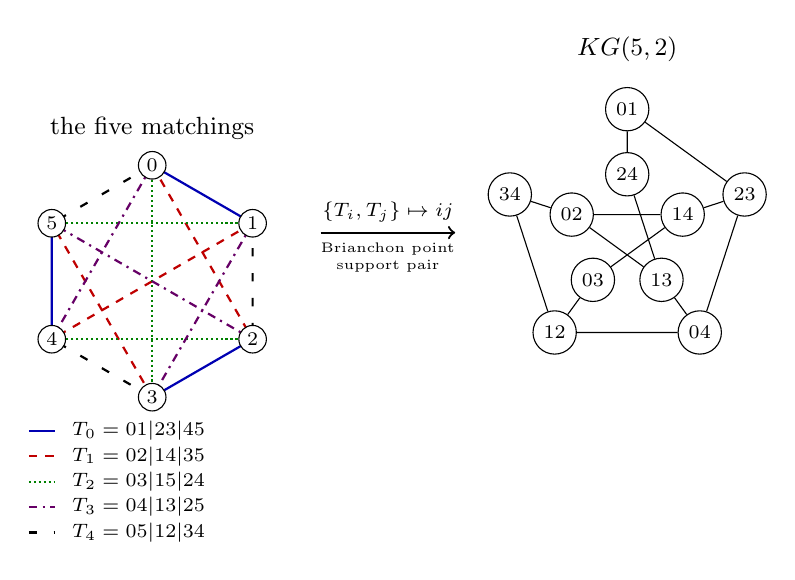
\begin{tikzpicture}[scale=0.95,
  vertex/.style={circle,draw,fill=white,inner sep=1.4pt,font=\scriptsize},
  pvertex/.style={circle,draw,fill=white,minimum size=5.5mm,inner sep=0pt,
                  font=\scriptsize}]
  % The invariant one-factorization on the six coordinate positions.
  \foreach \i/\a in {0/90,1/30,2/-30,3/-90,4/-150,5/150}
    \coordinate (v\i) at (\a:1.55);
  \draw[blue!70!black,thick] (v0)--(v1) (v2)--(v3) (v4)--(v5);
  \draw[red!75!black,thick,dashed] (v0)--(v2) (v1)--(v4) (v3)--(v5);
  \draw[green!50!black,thick,densely dotted] (v0)--(v3) (v1)--(v5) (v2)--(v4);
  \draw[violet!80!black,thick,dash dot] (v0)--(v4) (v1)--(v3) (v2)--(v5);
  \draw[black,thick,loosely dashed] (v0)--(v5) (v1)--(v2) (v3)--(v4);
  \foreach \i in {0,...,5} \node[vertex] at (v\i) {\i};
  \node[font=\small] at (0,2.05) {the five matchings};
  \begin{scope}[yshift=-2.0cm,font=\scriptsize]
    \draw[blue!70!black,thick] (-1.65,0)--(-1.3,0);
    \node[anchor=west] at (-1.2,0) {$T_0=01|23|45$};
    \draw[red!75!black,thick,dashed] (-1.65,-.34)--(-1.3,-.34);
    \node[anchor=west] at (-1.2,-.34) {$T_1=02|14|35$};
    \draw[green!50!black,thick,densely dotted] (-1.65,-.68)--(-1.3,-.68);
    \node[anchor=west] at (-1.2,-.68) {$T_2=03|15|24$};
    \draw[violet!80!black,thick,dash dot] (-1.65,-1.02)--(-1.3,-1.02);
    \node[anchor=west] at (-1.2,-1.02) {$T_3=04|13|25$};
    \draw[black,thick,loosely dashed] (-1.65,-1.36)--(-1.3,-1.36);
    \node[anchor=west] at (-1.2,-1.36) {$T_4=05|12|34$};
  \end{scope}

  \draw[->,thick] (2.25,.65)--(4.05,.65)
    node[midway,above,font=\scriptsize] {$\{T_i,T_j\}\mapsto ij$}
    node[midway,below,align=center,font=\tiny] {Brianchon point\\support pair};

  % Petersen graph on the two-subsets of {0,1,2,3,4}; adjacency is disjointness.
  \begin{scope}[xshift=6.35cm,yshift=.65cm]
    \node[pvertex] (p01) at (90:1.65) {01};
    \node[pvertex] (p23) at (18:1.65) {23};
    \node[pvertex] (p04) at (-54:1.65) {04};
    \node[pvertex] (p12) at (-126:1.65) {12};
    \node[pvertex] (p34) at (162:1.65) {34};
    \node[pvertex] (p24) at (90:.78) {24};
    \node[pvertex] (p14) at (18:.78) {14};
    \node[pvertex] (p13) at (-54:.78) {13};
    \node[pvertex] (p03) at (-126:.78) {03};
    \node[pvertex] (p02) at (162:.78) {02};
    \draw (p01)--(p23)--(p04)--(p12)--(p34)--cycle;
    \draw (p01)--(p24) (p23)--(p14) (p04)--(p13)
          (p12)--(p03) (p34)--(p02);
    \draw (p24)--(p13)--(p02)--(p14)--(p03)--cycle;
    \node[font=\small] at (0,2.45) {$KG(5,2)$};
  \end{scope}
\end{tikzpicture}
\caption{The five-matchings--Petersen dictionary. The line styles encode
the five self-polar triangles as perfect matchings of the six coordinates.
For each pair $\{T_i,T_j\}$, their union is an alternating six-cycle: its
opposite-edge matching gives a Brianchon point, and its alternating vertex
classes give a complementary support pair. Both are represented by the
Petersen vertex $ij$; adjacency means that the index pairs are disjoint.}
\label{fig:synthematic-petersen}
\end{figure}

\begin{proposition}[Brianchon--support dictionary]
\label{prop:brianchon-support}
Let $\mathcal T$ be the five self-polar triangles of Edge and
Dye~\cite{Edge1956,Dye1991}, regarded as five perfect matchings, and let
$\mathcal B(A)$ be the set of ten
Brianchon points of the Clebsch hexagon. For distinct $T,T'\in\mathcal T$,
the union $T\cup T'$ is an alternating six-cycle. Let $M(T,T')$ be the
perfect matching joining opposite vertices of this cycle. Let
$\beta(T,T')=\{S,S^{\mathsf c}\}$ be the unordered pair of alternating
vertex classes of the cycle.
For example, $T_0\cup T_1$ is the cycle
$0,1,4,5,3,2$, so $M(T_0,T_1)=05|13|24$ and
$\beta(T_0,T_1)=\{\{0,3,4\},\{1,2,5\}\}$.

The three chords indexed by $M(T,T')$ concur at a point $b(T,T')\in
\mathcal B(A)$. The maps
\[
 \binom{\mathcal T}{2}\longrightarrow\mathcal B(A),
 \qquad \{T,T'\}\longmapsto b(T,T'),
\]
and
\[
 \binom{\mathcal T}{2}\longrightarrow
 \bigl\{\{S,S^{\mathsf c}\}:|S|=3\bigr\},
 \qquad \{T,T'\}\longmapsto\beta(T,T'),
\]
are $A_5$-equivariant bijections. They identify the ten Brianchon points
with the ten complementary support pairs. Under this identification,
Petersen adjacency is disjointness of the corresponding two-element
subsets of $\mathcal T$.
\end{proposition}

\begin{proof}
The opposite-vertex matching is disjoint from $T$ and $T'$ and contains
one edge from each of the other three members of $\mathcal T$.
Hence $\{T,T'\}$ is recovered as the two members of $\mathcal T$ disjoint
from $M(T,T')$, so the ten triangle pairs give exactly the ten perfect
matchings outside $\mathcal T$. Applying the alternating-class rule to the
five displayed matchings gives ten distinct complementary support pairs,
hence all ten such pairs. Edge's Clebsch construction says that the
three chords of each such matching concur, at the ten distinct Brianchon
points~\cite[\S\S19--20,30]{Edge1956}. The bipartition bijection and
Petersen assertion are the alternating-cycle construction above.

The ten outside matchings give the ten triple concurrences. The remaining
fifteen intersections of disjoint chords have multiplicity one. Since every
step uses only the five invariant matchings and incidence, both bijections and their
compatibility with the support map are $A_5$-equivariant.
\end{proof}

\begin{corollary}[The decoder reconstructs the Brianchon configuration]
\label{cor:decoder-brianchon}
The ten projective directions having three nearest weight-two errors are
exactly the ten Brianchon points.  At each such direction the three error
supports are pairwise disjoint and hence form a perfect matching of the six
coordinates.  The ten matchings thereby recovered are precisely the ten
perfect matchings outside the five matchings in $\mathcal T$.
\end{corollary}

\begin{proof}
The three weight-two representations of a secant-index-three direction use
the three chords through it.  Proposition~\ref{prop:brianchon-support}
identifies the ten triple concurrences with the ten Brianchon points and
their chords with exactly the ten matchings outside $\mathcal T$.
\end{proof}

\begin{proposition}[Invariant support bipartition]
\label{prop:invariant-support-bipartition}
Only the bipartition is intrinsic: neither part has a canonical sign. The
twenty three-element coordinate supports split into two complementary
$A_5$-orbits $\mathcal O_+$ and $\mathcal O_-$ of size ten. For every
maximum-distance syndrome $s$, each support determines exactly one
weight-three leader of the coset $H^{-1}(s)$; hence that coset has ten
leaders supported in each class. Globally, the $2400$ minimum-weight
leaders split as $1200+1200$.

Every monomial automorphism of $C$ preserves this unordered bipartition.
The other coset in the exotic normalizer $N_{S_6}(A_5)\cong S_5$ exchanges
the two support classes, but its sixty elements are not automorphisms of the
displayed code. By
Proposition~\ref{prop:brianchon-support}, the ten complementary support
pairs are canonically both the two-subsets of the five self-polar triangles
and the ten Brianchon points.
\end{proposition}

\begin{proof}
The degree-six action of $A_5$ on the twenty three-subsets has two
ten-element orbits, exchanged by complementation. It preserves a unique
set of five perfect matchings, also preserved by
its full $S_5$ normalizer. The alternating-cycle construction of
Figure~\ref{fig:synthematic-petersen} is therefore equivariant, and the
outside normalizer coset exchanges the two support orbits. Fix a
maximum-distance syndrome $s$ and a three-support $S$. The three columns
indexed by $S$ are independent because $A$ is an arc, so they give a unique
coefficient vector representing $s$. None of its three coefficients can
vanish: otherwise $[s]$ would lie on a secant of $A$, contrary to maximum
distance. The resulting error vector therefore has weight three and is the
unique leader with support $S$. Finally, every monomial automorphism induces
a support permutation in $A_5$, by the exact sequence in
Section~\ref{sec:automorphisms}, and so preserves each support orbit. The
outside normalizer coset swaps the two orbits but cannot preserve $C$, even
after coordinate rescaling, because its support permutations lie outside
that quotient $A_5$.
\end{proof}

\section{Why \texorpdfstring{$q=11$}{q=11}}
\label{sec:why11}

Recall that $A$ is conic-filling when
$\cU(A)=\mathcal Q(\F_q)$ for some nonsingular conic $\mathcal Q$.
Equivalently,
$A\cap\mathcal Q(\F_q)=\varnothing$, its chords cover every point outside
$A\cup\mathcal Q(\F_q)$, and no chord meets $\mathcal Q(\F_q)$.
The conic-filling syndrome phenomenon of
Sections~\ref{sec:code}--\ref{sec:rigidity} is specific to $q=11$, even
without a symmetry hypothesis on the arc. A universal chord-defect
identity and the passant window leave only $q=9,11$; the former is excluded
by a classical exact-distance problem in the Sylvester graph.

\begin{lemma}[$q=9$ polarity graph]
\label{lem:q9-polarity}
For a nonsingular conic $\cC\subset\PG(2,9)$, let $\Sigma$ be the graph on
the $36$ internal points in which
\[
 P\sim Q\quad\Longleftrightarrow\quad Q\in P^\perp
\]
for the conic polarity. Then $\Sigma$ is the Sylvester graph, with
intersection array
\[
 \{5,4,2;1,1,4\}.
\]
For distinct internal points $P,Q$, the line $PQ$ is passant to $\cC$ if
and only if $P$ and $Q$ are at distance two in $\Sigma$, and the graph
joining pairs at distance two has clique number
\[
 \omega(\Sigma_2)=5.
\]
\end{lemma}

\begin{proof}
Counting internal points on polar lines and their intersections gives
$b_0=5$, $b_1=4$, $b_2=2$, $c_1=c_2=1$, and $c_3=4$, hence the displayed
intersection array. This is the Sylvester graph
\cite[\S13.1.2]{BrouwerCohenNeumaier1989}; uniqueness for this intersection
array is proved in~\cite[Thm.~6]{JurisicVidali2019}.

For distinct internal points $P,Q$, put
$R=P^\perp\cap Q^\perp=(PQ)^\perp$. If $PQ$ is passant, then its pole $R$
is internal and adjacent to both $P$ and $Q$; since the intersection array
has $a_1=0$, these vertices are at distance two. Conversely, a common
neighbor of $P$ and $Q$ must equal $R$, so distance two makes the pole of
$PQ$ internal and hence makes $PQ$ passant. The final value is
$\operatorname{eq}_2(\Sigma)=5$ in
\cite[Table~1]{AbiadJabalAmeliReijnders2025}.
\end{proof}

\begin{theorem}[Uniqueness of $q=11$]
\label{thm:why11}
Let $q$ be a prime power. If a six-arc $A\subset\PG(2,q)$ satisfies
$\cU(A)=\cC(\F_q)$ for some nonsingular conic $\cC$, then $q=11$.
At $q=11$ every such $A$ is projectively equivalent to the
Clebsch hexagon.
\end{theorem}

\begin{proof}
Corollary~\ref{cor:conic-filling-window} gives $q\ge9$ and
$c(A)=(q-6)(q-9)$ with $0\le c(A)\le15$. Thus the only prime-power
candidates are $q=9,11$: $q=10$ is not a prime power, and every
$q\ge12$ gives $c(A)\ge18$.

It remains to exclude $q=9$. Since every point of $\cC$ is uncovered, no
chord of $A$ meets $\cC$; every chord is therefore passant. A point off
$\cC$ lies on five passants if it is internal and four if it is external,
so the five chords through each vertex force all six vertices of $A$ to be
internal. Lemma~\ref{lem:q9-polarity} would then make $A$ a
six-clique in the distance-two graph of the Sylvester graph, whose clique
number is five. This is impossible.

Therefore $q=11$. The final assertion follows from
Theorem~\ref{thm:rigidity}, which puts every matching $q=11$ representative
in the single Clebsch orbit.
\end{proof}

\begin{proposition}[The Clebsch-family uncovered formula]
\label{prop:clebsch-family-uncovered}
Let $K$ be a Clebsch hexagon over $\F_q$; equivalently, $K$ is a six-arc
with ten Brianchon points. By Dye's existence theorem, the characteristic
is not two and $5$ has a square root in $\F_q$, possibly zero in
characteristic five. Then
\[
 |\cU(K)|=q^2-14q+45.
\]
If $q\equiv3\pmod4$ and $\cC$ is Dye's associated conic, then
$\cC(\F_q)\subseteq\cU(K)$ and
\[
 |\cU(K)\setminus\cC(\F_q)|=(q-4)(q-11).
\]
In particular, among Clebsch hexagons in this congruence class, the
associated conic is the complete projective deep-hole syndrome locus if and
only if $q=11$.
\end{proposition}

\begin{proof}
Dye defines a Clebsch hexagon by the occurrence of exactly ten Brianchon
points, and his Theorem~1 classifies their existence and projective orbit
\cite[p.~271; Theorem~1, pp.~275--276]{Dye1991}. These points are precisely
the off-vertex
triple-chord concurrences counted by $c(K)$. Thus $c(K)=10$, and
Theorem~\ref{lem:chord-defect} gives
\[
 |\cU(K)|=q^2-14q+55-10=q^2-14q+45.
\]
Dye also shows that the edges of $K$ are non-secants of the associated conic
when $q\equiv3\pmod4$~\cite[discussion preceding Theorem~6,
pp.~281--282]{Dye1991}. Hence every rational point of $\cC$ is uncovered.
Subtracting $|\cC(\F_q)|=q+1$ from the first formula gives
\[
 q^2-15q+44=(q-4)(q-11).
\]
The factor vanishes only at $q=4$ and $q=11$, and the stated congruence
leaves only $q=11$. Conversely, Clebsch hexagons exist over $\F_{11}$ by
Dye's Theorem~1, and the inclusion above is then an equality because both
sets have twelve points.
\end{proof}

\begin{remark}[Three Clebsch-family regimes]
The polynomial $q^2-14q+45=(q-5)(q-9)$ vanishes exactly at $q=5,9$.
The root $q=5$ lies in characteristic five, where the
associated-conic construction of Definition~\ref{def:hexagon} is
not available. At $q=9$, however, Dye's construction applies:
$5=-1$ is a square in $\F_9$, and the characteristic is three. Thus the
formula recovers a complete Clebsch six-arc at $q=9$. Independently,
Theorem~\ref{thm:why11}
excludes every six-arc over $\F_9$ from conic filling by the Sylvester-graph
clique bound. At $q=11$ the uncovered locus is instead exactly the
associated conic.

At $q=19$, the same icosahedral construction still produces a Clebsch
six-arc disjoint from its associated conic, but the covering fails. The
twenty conic points remain uncovered~\cite[p.~281]{Dye1991}, while
Proposition~\ref{prop:clebsch-family-uncovered} gives
\[
 |\cU(A)|=140=20+120.
\]
Thus $120=(19-4)(19-11)$ additional points escape all fifteen secants, and
$\cU(A)$ lies on no conic. The configuration persists; exact conic filling
is what the factorization isolates at $q=11$.
\end{remark}

\subsection{The small-arc boundary}

The chord moments reduce the neighboring cases through eight points to a
finite list of fields. Exact terminal enumeration excludes the remaining
seven- and eight-point cases.

\begin{theorem}[Conic-filling loci through eight points]
\label{thm:small-k-conic-filling}
Let $A$ be a $k$-arc in $\PG(2,q)$, where $q$ is a prime power and
$4\le k\le8$, and suppose that $\cU(A)$ is the full set of
$\F_q$-rational points of a nonsingular conic. Then
\[
 (k,q)=(4,5)\qquad\text{or}\qquad(k,q)=(6,11).
\]
In the first case $A$ is a projective four-frame; in the second it is a
Clebsch hexagon. Conversely, both cases occur.

Moreover, for each $q\in\{13,17,19\}$, an arc all of whose chords are
passant to a fixed nonsingular conic has at most six points, and this bound
is attained.
\end{theorem}

\begin{proof}[Proof with exhaustive finite verification]
For $k=4$, Corollary~\ref{cor:conic-filling-window} gives
$5\le q<6$, hence $q=5$. Every four-arc is a projective frame, and for the
standard frame a direct
substitution gives
\[
 \cU(A)=V(X^2+Y^2+Z^2+XY+XZ+YZ),
\]
where $V(f)$ denotes the projective zero set of $f$; this is a nonsingular
six-point conic. For $k=5$, the theorem gives
$|\cU(A)|=q^2-9q+21$; equality with $q+1$ would require
$q^2-10q+20=0$, which has no integral root. The case $k=6$ is
Theorem~\ref{thm:why11} together with Theorem~\ref{thm:rigidity}.

For $k=7$, Theorem~\ref{lem:chord-defect} gives
\[
 |\cU(A)|=q^2-20q+120-n_3.
\]
If this equals $q+1$, then
\[
 n_3=q^2-21q+119,\quad
n_2=105-3n_3,\quad
 n_1=3(q^2-14q+42).
\]
The conic-filling window and quadratic barrier give $q\ge11$ and
$q^2-21q+84\le0$, hence $q\le15$. Thus only the prime powers $q=11,13$
remain, with forced spectra
$(n_1,n_2,n_3)=(27,78,9)$ and $(87,60,15)$ respectively. An exhaustive
four-frame-normalized enumeration now supplies the finite exclusion. It
finds $10232$ distinct normalized seven-arcs at $q=11$, of which $140$ have
$|\cU(A)|=q+1$, and $53960$ at $q=13$, of which $1680$ have that size.
Every seven-arc is reached because it contains a four-frame; extending each
normalized six-arc by its uncovered points produces every resulting
seven-arc exactly three times, according to which non-frame point is
deleted. For all $1820$ candidates of the required size, the quadratic
evaluation matrix has full rank six, so none lies on a conic.

Finally let $k=8$. The conic-filling window and its quadratic inequality
give $q\ge13$ and $q^2-28q+125\le0$, hence $q\le22$. The prime powers in
this interval that are odd are exactly $13,17,19$.

It remains to exclude these three fields. By projective equivalence fix the
conic $XZ=Y^2$, whose stabilizer is the symmetric-square image of
$\operatorname{PGL}(2,q)$. Its complement has $q^2$ points. In the
terminology of Blokhuis, Seress, and Wilbrink, a set whose pairwise joins
are passant is an exterior set of the conic
\cite[pp.~143,146]{BSW1992}; its vertices may have either internal or
exterior point type. Every conic-filling arc is such an exterior set.

There is already a structural reduction at $q=13$. An exterior point lies
on only $(q-1)/2=6$ passants, fewer than the seven distinct chords through
a vertex of an eight-arc. Hence every vertex would be internal. Each
internal point lies on exactly $(q+1)/2=7$ passants, so its seven chords
would exhaust its complete passant pencil.

For the remaining finite step, join two off-conic points when their line is
passant. The desired eight-arc would be an eight-clique in this graph, with
collinear triples forbidden.

An exact orbit search gives the complete reduction
\[
\begin{array}{c|c|c|c}
q&\text{off-conic points}&\text{passant edges}&
 \operatorname{PGL}(2,q)\text{-orbits on edges}\\ \hline
13&169&7098&10\\
17&289&20808&13\\
19&361&32490&15.
\end{array}
\]
For one representative of each edge orbit, the search extends partial arcs
and identifies states under the setwise stabilizer of the root edge.
Canonical keys are the lexicographically least sorted point lists in each
stabilizer orbit. Every candidate is reached: it contains a passant edge,
that edge is carried to one of the listed representatives, and the remaining
points are then among the enumerated extensions. In all three fields the
largest partial arc has size six. Thus there is no seven-point arc with all
chords passant, and in particular no conic-filling eight-arc. A separate
replay verifies the edge-orbit partition and repeats the extension search by
ordered backtracking without stabilizer identification. Its certificates
give an explicit six-point witness in every field, proving sharpness.
\end{proof}

In coding terms, let $C$ be a projective $[k,k-3,4]_q$ MDS code with
$4\le k\le8$. If its projective distance-three syndrome locus is a
nonsingular conic, then, up to monomial equivalence, $C$ is the
$[4,1,4]_5$ frame code or the $[6,3,4]_{11}$ Clebsch code. Both codes have
the stated syndrome locus.

Thus, for each fixed arc size, only finitely many field orders can admit
conic filling; the classification is complete through eight points.

\section{Verification architecture}
\label{sec:verification}

\begingroup
\setlength{\emergencystretch}{1em}
Tables~\ref{tab:verification} and~\ref{tab:replays} separate the adopted
claims, mathematical input, kernel-checked formal proof, and exhaustive
finite enumeration. Here
``kernel-checked'' means that Lean's trusted kernel checks the stated
implication; executable replays instead enumerate the finite search space
with exact arithmetic. The separately distributed formal source tree is
pinned at commit
\path{6d4766d1ea5e9a36f1a507e549c223416a6b506f}; it uses Lean 4.32.0-rc1
and Mathlib commit
\path{571b8a8e54219b4d393f75f4b8653fac08197fcc}. Manifest, release, and
executable checker paths are relative to this paper root; Lean paths are
relative to the formal source root.
These tables are the paper's consolidated proof-mode ledger; the theorem
statements and proofs do not carry separate ``Proof mode'' tags.
The claim-by-claim manifest is \path{verification/trust_manifest.json}; the
aggregate formal gate is
\path{RelativeConicArcs/Gates/ClebschRigidityTrust.lean}. The clean replay
entry point is \path{verification/verify_release.py}.

The shared formal source is distributed in the
\href{https://github.com/tavisrudd/finitegeom}{\texttt{finitegeom} GitHub
repository} and is pinned above to an exact commit. With a checkout of that
repository, run from this paper root:
\begin{verbatim}
nix develop --command python3 verification/verify_release.py \
  --lean-root /absolute/path/to/finitegeom
\end{verbatim}
The SHA-256 digest of \path{verification/checker_outputs.json} is
\begin{center}
\small\path{b5577fa19c35992950faf486cac33df5de523ff05162e6fa42ecd886302fdcbc}.
\end{center}
The SHA-256 digest of
\path{RelativeConicArcs/Gates/ClebschRigidityTrust.lean} is
\begin{center}
\small\path{dce51b42bfb384950bbffa756a87c3aabccfda03502d19545988f52aca32cb69}.
\end{center}
\par
\endgroup

\begin{table}[H]
\centering
\footnotesize
\begin{tabular}{@{}>{\raggedright\arraybackslash}p{0.22\textwidth}
                    >{\raggedright\arraybackslash}p{0.31\textwidth}
                    >{\raggedright\arraybackslash}p{0.37\textwidth}@{}}
\toprule
Result & Mathematical input & Kernel-checked formalization \\
\midrule
$A_5$ orbits and syndrome conic
& Dye for the orbit data; chord defect and exteriority for the conic equality
& \path{RelativeConicArcs/Q11A5PointOrbits.lean};
\path{RelativeConicArcs/Q11Coding.lean} \\
Decoding and Brianchon supports
& arc--coset dictionary; Edge--Dye incidence
& \path{RelativeConicArcs/Q11DecodingSynthesis.lean} \\
Invariant support bipartition
& Edge--Dye triangles; incidence reconstruction
& --- \\
Rigidity theorem
& line bound; chord defect; Dye's \S2.2 and Theorem~1(ii)
& \path{RelativeConicArcs/Q11DyeAxioms.lean};
\path{RelativeConicArcs/Q11DyeConsequences.lean};
\path{RelativeConicArcs/SixArcDefectBridge.lean} \\
Universal defect and conic-filling window
& two chord moments; passant counts
& six-arc specialization only:
\path{RelativeConicArcs/ClebschChordDefect.lean} \\
Gap and low-degree loci
& finite linear algebra over $\F_{11}$
& --- \\
Uniqueness of $q=11$
& conic-filling window; cited Sylvester bound
& \path{RelativeConicArcs/ClebschChordDefect.lean};
\path{RelativeConicArcs/Q9Sylvester.lean} \\
Clebsch-family formula
& Dye's ten Brianchon points and edge criterion
& --- \\
Classification through eight points
& universal chord moments and defect bound
& \path{RelativeConicArcs/SmallKChordMoments.lean};
\path{RelativeConicArcs/SmallKGeometricBridge.lean}
\\
\bottomrule
\end{tabular}
\caption{Mathematical and formal dependencies of the principal results.}
\label{tab:verification}
\end{table}

The gap/low-degree result and the Clebsch-family formula have no Lean
coverage. Their executable routes in Table~\ref{tab:replays} are
load-bearing checks, not independent supplements to a formal proof.

\begin{table}[H]
\centering
\footnotesize
\begin{tabular}{@{}>{\raggedright\arraybackslash}p{0.27\textwidth}
                    >{\raggedright\arraybackslash}p{0.65\textwidth}@{}}
\toprule
Result & Exhaustive or independent executable check \\
\midrule
$A_5$ orbits and syndrome conic
& \path{check_rigidity_degenerate_conic.py} (syndrome-conic clause) \\
Decoding and Brianchon supports
& \path{check_decoding.py} \\
Invariant support bipartition
& \path{check_chirality.py}; \path{check_code_automorphisms.py} \\
Rigidity theorem
& \path{check_rigidity_degenerate_conic.py};
$1548$-representative frame-normalized enumeration \\
Universal defect and conic-filling window
& conceptual double counting; no separate executable check \\
Gap and low-degree loci
& \path{check_global_conic_gap.py}; \path{check_low_degree_loci.py} \\
Uniqueness of $q=11$
& \path{check_small_q_uniqueness.py}; independent $q=9$ construction \\
Clebsch-family formula
& \path{check_q19_nonexample.py} \\
Classification through eight points
& \path{check_small_k_conic_filling.py};
\path{verification/c605_verify.py} \\
\bottomrule
\end{tabular}
\caption{Executable checks, separate from the formal dependencies in
Table~\ref{tab:verification}.}
\label{tab:replays}
\end{table}

The formal development axiomatizes exactly two classical inputs from Dye:
the ten-point Brianchon bound from \S2.2, page~275, and the projective
equality classification from Theorem~1(ii), page~275.
The line bound and chord-defect identity are proved independently. At
$q=11$, the finite census also checks the imported numerical conclusion:
$|\cU(A)|=12=22-10$ is equivalent to the maximal value $c(A)=10$.

\section{Conclusion}

For every fixed arc size, the universal defect identity bounds the field
orders that can admit conic filling. It reduces both the isolation of
$q=11$ and the classification for $4\le k\le8$ to bounded terminal cases.
The two-sided conic-filling window first reduces the eight-point case to
three fields; exact orbit search excludes all three.
The numerical window is nonempty for
every $k\ge4$ and has width
$\binom{k}{2}-(2k-3)=\binom{k-2}{2}$; it is sharp at $k=4$, where its sole
integer is $q=5$ and conic filling occurs. The Clebsch code realizes a
different kind of sharpness:
covering-radius data recover geometry that was not built into the code,
forcing the Clebsch hexagon and hence its $A_5$ symmetry. A line bound and
the defect identity reduce that rigidity to Dye's equality case;
enumeration is reserved for the low-degree strengthening, the numerical
gap, and the terminal $k=7,8$ exclusions.

More generally, which odd prime powers in the
quadratically widening window admit conic-filling arcs? A second problem is
to connect fixed-$k$ rigidity with the large-arc conic-forcing regime. Both
ask how far a syndrome locus can reconstruct the projective system that
produced it.

The same questions have useful algebraic and spectral forms. The terminal
exclusions are clique problems in the passant graph, suggesting
association-scheme bounds in place of orbit search. The degree-three
recognition theorem asks which Hilbert functions of uncovered loci determine
an arc, while the decoder results ask when coset-leader support data alone
reconstruct a projective code.

\bibliographystyle{plain}
\begin{thebibliography}{99}

\bibitem{BSW1992}
A.~Blokhuis, Á.~Seress, and H.~A.~Wilbrink,
\newblock Characterization of complete exterior sets of conics,
\newblock \emph{Combinatorica} \textbf{12}(2) (1992), 143--147.
\newblock doi:10.1007/BF01204717.

\bibitem{BicharaKorchmaros1982}
A.~Bichara and G.~Korchm\'aros,
\newblock Note on $(q+2)$-sets in a Galois plane of order $q$,
\newblock in \emph{Combinatorial and Geometric Structures and Their
Applications}, Annals of Discrete Mathematics \textbf{14}, North-Holland,
1982, 117--121.
\newblock doi:10.1016/S0304-0208(08)73588-6.

\bibitem{Clebsch1871}
A.~Clebsch,
\newblock Ueber die Anwendung der quadratischen Substitution auf die
Gleichungen 5-ten Grades und die geometrische Theorie des ebenen Fünfseits,
\newblock \emph{Mathematische Annalen} \textbf{4} (1871), 284--345.

\bibitem{Edge1956}
W.~L.~Edge,
\newblock Conics and orthogonal projectivities in a finite plane,
\newblock \emph{Canadian Journal of Mathematics} \textbf{8} (1956), 362--382.

\bibitem{DrakeKeating2004}
D.~A.~Drake and K.~Keating,
\newblock Ovals and hyperovals in Desarguesian nets,
\newblock \emph{Designs, Codes and Cryptography} \textbf{31} (2004),
195--212.
\newblock \url{https://doi.org/10.1023/B:DESI.0000015883.89954.80};
arXiv:math/0202115.

\bibitem{ChengMurray2007}
Q.~Cheng and E.~Murray,
\newblock On deciding deep holes of Reed--Solomon codes,
\newblock in \emph{Theory and Applications of Models of Computation (TAMC
2007)}, Lecture Notes in Computer Science \textbf{4484}, Springer, 2007,
296--305.

\bibitem{DMP2021}
A.~A.~Davydov, S.~Marcugini, and F.~Pambianco,
\newblock On the weight distribution of the cosets of MDS codes,
\newblock \emph{Advances in Mathematics of Communications} \textbf{17}(5)
(2023), 1115--1138.
\newblock arXiv:2101.12722v2.
\newblock (Numbered results are cited by their arXiv~v2 numbering.)

\bibitem{BallLavrauw2019}
S.~Ball and M.~Lavrauw,
\newblock Arcs in finite projective spaces,
\newblock \emph{EMS Surveys in Mathematical Sciences} \textbf{6} (2019),
33--45.
\newblock arXiv:1908.10772.

\bibitem{AbiadJabalAmeliReijnders2025}
A.~Abiad, A.~Jabal Ameli, and L.~Reijnders,
\newblock The clique number of the exact distance $t$-power graph:
complexity and eigenvalue bounds,
\newblock \emph{Discrete Applied Mathematics} \textbf{363} (2025), 55--70.
\newblock doi:10.1016/j.dam.2024.11.032.

\bibitem{BrouwerCohenNeumaier1989}
A.~E.~Brouwer, A.~M.~Cohen, and A.~Neumaier,
\newblock \emph{Distance-Regular Graphs},
\newblock Ergebnisse der Mathematik und ihrer Grenzgebiete, vol.~18,
Springer-Verlag, Berlin, 1989.

\bibitem{JurisicVidali2019}
A.~Juri\v{s}i\'c and J.~Vidali,
\newblock The Sylvester graph and Moore graphs,
\newblock \emph{European Journal of Combinatorics} \textbf{80} (2019),
184--193.
\newblock doi:10.1016/j.ejc.2018.02.018.

\bibitem{Dye1991}
R.~H.~Dye,
\newblock Hexagons, conics, $A_5$ and $\mathrm{PSL}_2(K)$,
\newblock \emph{Journal of the London Mathematical Society} (2) \textbf{44}
(1991), 270--286.
\newblock doi:10.1112/jlms/s2-44.2.270.

\bibitem{GuruswamiVardy2005}
V.~Guruswami and A.~Vardy,
\newblock Maximum-likelihood decoding of Reed--Solomon codes is NP-hard,
\newblock \emph{IEEE Transactions on Information Theory} \textbf{51}(7)
(2005), 2249--2256.

\bibitem{Hirschfeld1998}
J.~W.~P.~Hirschfeld,
\newblock \emph{Projective Geometries over Finite Fields}, second edition,
\newblock Oxford University Press, 1998.

\bibitem{MendelsohnRosa1985}
E.~Mendelsohn and A.~Rosa,
\newblock One-factorizations of the complete graph---a survey,
\newblock \emph{Journal of Graph Theory} \textbf{9}(1) (1985), 43--65.
\newblock doi:10.1002/jgt.3190090104.

\bibitem{NgWild2001}
S.-L.~Ng and P.~R.~Wild,
\newblock On $k$-arcs covering a line in finite projective planes,
\newblock \emph{Ars Combinatoria} \textbf{58} (2001), 289--300.

\bibitem{SadehThesis1984}
A.~R.~Sadeh,
\newblock \emph{Classification of $k$-arcs in $\PG(2,11)$ and cubic
surfaces in $\PG(3,11)$},
\newblock D.Phil.\ thesis, University of Sussex, 1984.

\bibitem{StormeThas1991}
L.~Storme and J.~A.~Thas,
\newblock Generalized Reed--Solomon codes and normal rational curves: an
improvement of results by Seroussi and Roth,
\newblock in \emph{Advances in Finite Geometries and Designs}, Oxford
University Press, 1991, 369--389.

\bibitem{SVM1995}
L.~Storme and H.~Van~Maldeghem,
\newblock Primitive arcs in $\PG(2,q)$,
\newblock \emph{Journal of Combinatorial Theory, Series A} \textbf{69}
(1995), 200--216.
\newblock doi:10.1016/0097-3165(95)90051-9.

\bibitem{ZWK2020}
Y.~Zhang, D.~Wan, and K.~Kaipa,
\newblock Deep holes of projective Reed--Solomon codes,
\newblock \emph{IEEE Transactions on Information Theory} \textbf{66}(4)
(2020), 2392--2401.
\newblock arXiv:1901.05445.

\end{thebibliography}

\end{document}
